% Configuration
\documentclass[12pt,a4paper]{article}
\usepackage[a4paper, top=2.0cm, bottom=2.0cm, right=2.0cm, left=2.0cm, nohead]{geometry}
\usepackage[utf8]{inputenc}
\usepackage{czech}
\usepackage{multicol}
\usepackage{graphicx}

% Disables some warning messages
\sloppy
\hbadness 10000

% Basic document information
\title{Protokol do předmětu HSC}
\author{Petr Zemek, xzemek02@stud.fit.vutbr.cz}

\begin{document}

% Header
\noindent
\begin{small}Projekt do předmětu Hardware/Software Codesign \\ 28.~prosince~2008\end{small} \\

% Title
\begin{center}
	\begin{large}\textbf{Vestavěný systém pro filtraci a kompresi obrazu}\end{large} \\
	\vspace{0.4cm}
	Petr Zemek \\
	\textit{xzemek02@stud.fit.vutbr.cz} \\
	\textit{Fakulta Informačních Technologií, Brno} \\
\end{center}

\subsection*{1 Časová analýza algoritmu}

Kolik procent času strávil procesor ve funkci z celkové doby výpočtu.

%median_quick 79.78 77.85 76.64 77.39 77.54 79.24 77.13 81.44 77.18 78.42 => 78.26
%system_input 16.31 17.81 19.59 17.86 18.67 17.78 19.13 16.53 18.85 18.63 => 18.12
%processing 2.55 2.51 1.99 2.32 2.22 1.64 1.85 0.86 2.55 1.25 => 1.97
%rle_komprese 1.63 1.98 1.82 2.62 1.61 1.61 2.11 1.38 1.45 1.84 => 1.80
%system_output 0.09 0.12 0.35 0.18 0.20 0.09 0.20 0.15 0.27 0.16 => 0.18

\begin{multicols}{2}
	\noindent
	\vspace*{0.2cm}
	\begin{center}
		\begin{tabular}{| l | l |}
		\hline
		Název funkce & \% času \\
		\hline
		\texttt{median\_quick} & $78.26$ \\
		\texttt{system\_input} & $18.12$ \\
		\texttt{processing} & $1.97$ \\
		\texttt{rle\_komprese} & $1.80$ \\
		\texttt{system\_output} & $0.18$ \\
		\hline
		\end{tabular}
	\end{center}

	\noindent
	\begin{center}
		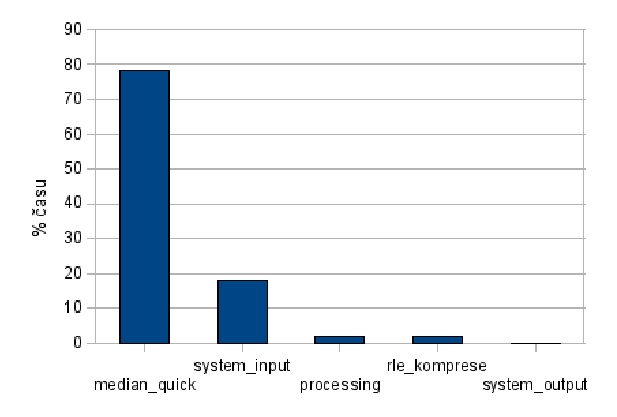
\includegraphics[width=8.0cm,keepaspectratio]{graph}
	\end{center}
\end{multicols}

\subsection*{2 Průměrná doba zpracování obrazu}

%-------------------------------------------------------------------------------
% SW reseni
%-------------------------------------------------------------------------------
% Prumerna doba zpracovani jednoho bodu:
% 1930-370 = 1560
% 708730-699490 = 9240
% 1097050-1088770 = 8280
% 1669530-1666050 = 3480
% 2436250-2434690 = 1560
% 2440690-2436250 = 4440
% 3162170-3160610 = 1560
% 3306210-3299370 = 6840
% 3373410-3365610 = 7800
% 1591050-1584690 = 6360
% (1560+9240+8280+3480+1560+4440+1560+6840+7800+6360)/10.0 = 5112 ns
%
% Pocet cyklu:
% 5112 / 20 ns = 255
%
% Pocet bodu za vterinu:
% 1 / (5112*10^-9) = 195618.15
%
% Pocet snimku za vterinu pro jednotliva rozliseni:
% 195618.20 / (160*100) = 5.98
% 195618.20 / (320*200) = 3.06
% 195618.20 / (640*480) = 0.64
% 195618.20 / (800*600) = 0.41
% 195618.20 / (1024*768) = 0.25
% 195618.20 / (1280*1024) = 0.15
% 195618.20 / (1600*1200) = 0.10
%
%-------------------------------------------------------------------------------
% HW reseni
%-------------------------------------------------------------------------------
% Prumerna doba zpracovani jednoho bodu:
% 890-370 = 520
% 22930-22410 = 520
% 635530-635010 = 520
% 570490-569970 = 520
% 506690-506170 = 520
% 466330-465810 = 520
% 413530-413010 = 520
% 366650-366130 = 520
% 343210-342690 = 520
% 302210-301690 = 520
% (520*10)/10 = 520 ns
%
% Pocet cyklu:
% 520 / 20 ns = 26
%
% Pocet bodu za vterinu:
% 1 / (520*10^-9) = 1923076.92
%
% Pocet snimku za vterinu pro jednotliva rozliseni:
% 1923076.92 / (160*100) = 120.20
% 1923076.92 / (320*200) = 30.05
% 1923076.92 / (640*480) = 6.26
% 1923076.92 / (800*600) = 4.00
% 1923076.92 / (1024*768) = 2.45
% 1923076.92 / (1280*1024) = 1.48
% 1923076.92 / (1600*1200) = 1.00

\begin{multicols}{2}
	\noindent
	Průměrná doba, průměrný počet cyklů pro zpracování jednoho bodu snímku a
	kolik bodů za vteřinu je takto možné zpracovat u obou řešení:
	\vspace*{0.2cm}
	\begin{center}
		\begin{tabular}{| l | l | l |}
		\hline
		 & SW & HW \\
		\hline
		Průměrná doba & 5112 ns & 520 ns \\
		Průměrný počet cyklů & 255 & 26 \\
		Počet bodů za vteřinu & 195618.20 & 1923076.92 \\
		\hline
		\end{tabular}
	\end{center}

	$ $ \newline

	\noindent
	Kolik snímků za vteřinu jsou schopné obě řešení zpracovat v daných rozlišeních:
	\vspace*{0.2cm}
	\begin{center}
		\begin{tabular}{| l | l | l |}
		\hline
		 & SW & HW \\
		\hline
		160x100 & 5.98 & 120.20 \\
		320x200 & 3.06 & 30.05 \\
		640x480 & 0.64 & 6.26 \\
		800x600 & 0.41 & 4.00 \\
		1024x768 & 0.25 & 2.45 \\
		1280x1024 & 0.15 & 1.48 \\
		1600x1200 & 0.10 & 1.00 \\
		\hline
		\end{tabular}
	\end{center}
\end{multicols}

\subsection*{3 Doba potřebná pro zpracování jednoho bodu}

Doba, za kterou musí systém zpracovat jeden bod při rozlišení obrazu 160x100, 320x200,
640x480, 800x600, 1024x768, 1280x1024 a 1600x1200 a rychlosti 5 snímků za vteřinu.

\begin{multicols}{2}
	\noindent
	\vspace*{0.2cm}
	\begin{center}
		\begin{tabular}{| l | l | l |}
		\hline
		Rozlišení & Doba \\
		\hline
		160x100 & $12.500\,\mu{s}$ \\
		320x200 & $3.125\,\mu{s}$ \\
		640x480 & $0.651\,\mu{s}$ \\
		800x600 & $0.417\,\mu{s}$ \\
		1024x768 & $0.254\,\mu{s}$ \\
		1280x1024 & $0.153\,\mu{s}$ \\
		1600x1200 & $0.104\,\mu{s}$ \\
		\hline
		\end{tabular}
	\end{center}

	\noindent
	\begin{center}
		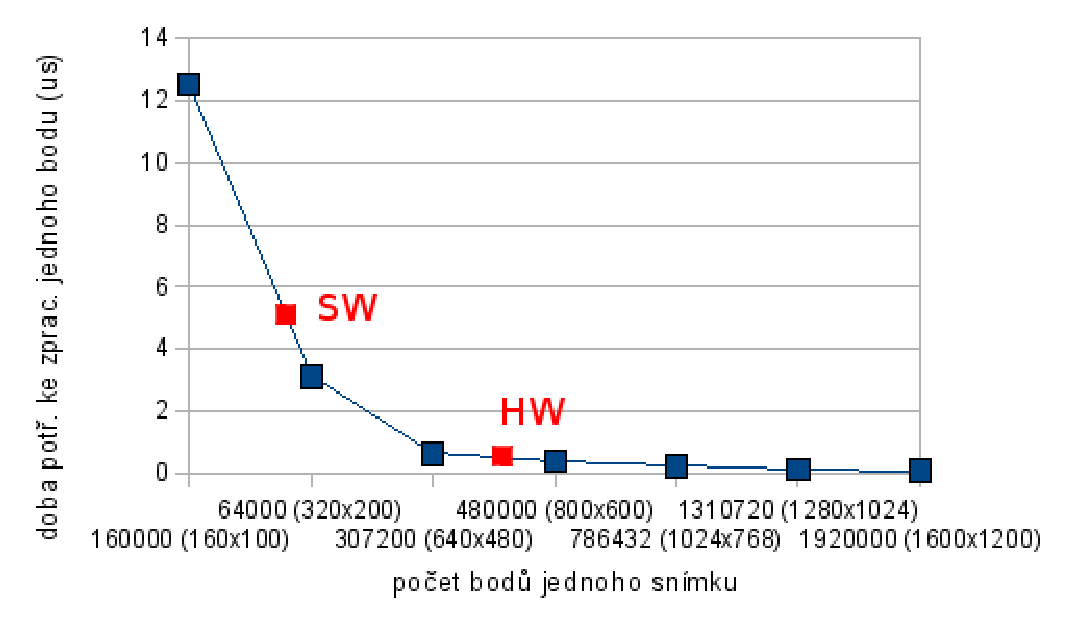
\includegraphics[width=8.0cm,keepaspectratio]{graph2}
	\end{center}
\end{multicols}

\subsection*{4 Využitá plocha na čipu a maximální frekvence}

\noindent
Maximální frekvence: 99.354 MHz

\noindent
Zaplnění FPGA čipu: 70\% (539 slices ze 768)

\subsection*{5 Shrnutí}

Během práce na projektu byly dodrženy všechny požadavky ze zadání.
Po implementaci čistě softwareové realizace projektu se ukázalo, že rychlost
zpracování je nedostatečná (systém nebyl schopen zpracovat ani jediný snímek
při rozlišení 640x480). Dle výsledků z profileru jsem se rozhodl hardwareově
akcelerovat výpočet mediánu, protože tato činnost zabírala procesoru skoro 80\%
času. S hardwareovou implementací již byl systém schopen zpracovat zadaných
5 snímků za vteřinu při rozlišení 640x480. V případě, že by bylo třeba systém
ještě urychlit, pak by se mohl hardwareově akcelerovat výpočet RLE, což by ovšem
způsobilo nárůst využitého místa na čipu.
Systém byl nakonec úspěšně otestován na přípravku FITKit s využitím
vizualiace pomocí VGA výstupu.
Zaplněno bylo 70\% místa na čipu, což by mohlo způsobit problémy, pokud by bylo
třeba systém rozšířit o další funkčnost (např. přidání dalšího filtrování).
Pro výpočet ceny a spotřeby mého řešení jsem neměl dostatek informací.

\end{document}
